\chapter{Exploratory Data Analysis}
\section{Data description}
The data were received as an email attachment from our contact at Glaxo Smithkline. The attachment was a SAS data set which was able to be read into R by first exporting from SAS in dbf format and then read into R using the \texttt{read.dbf} function.
Table \ref{rdata} shows the data as an R data frame. 
\begin{table}[h]
\caption{Data as an R data frame}\label{rdata}
\begin{boxedverbatim}
    CENTREID SUBJID SEX                    plantm   acttm  parct trt trttxt
1        001     54   M                  PRE-DOSE -2.8333  14092   A  alone
2        001     54   M  2 HOURS AFTER FIRST DOSE  2.0333   7592   A  alone
3        001     54   M  4 HOURS AFTER FIRST DOSE  4.0500   1170   A  alone
4        001     54   M  6 HOURS AFTER FIRST DOSE  6.0000     52   A  alone
5        001     54   M  8 HOURS AFTER FIRST DOSE  8.0500      0   A  alone
\end{boxedverbatim}
\end{table}

The columns are:
\begin{itemize}
\item\texttt{CENTREID} - The centre at which the study was undertaken, either centre '001' or '002'.
\item\texttt{SUBJID} - An identifier for each subject (patient) participating in the trial. There are 43 subjects.
\item\texttt{SEX} - The sex of each subject, either 'M' or 'F'.
\item\texttt{plantm} - The planned time of taking a blood sample for measuring parasite load, either 'PRE-DOSE' i.e. before the drug treatment is administered, or 'n HOURS AFTER FIRST DOSE'.
\item\texttt{acttm} - The actual time in hours that the blood sample was taken relative to the time the treatment was administered, hence all pre-dose times are negative.
\item\texttt{parct} - The parasite count per $\mu L$ of blood.
\item\texttt{trt} - An indicator of which treatment was used 'A' or 'B'.
\item\texttt{trttxt} - A description of treatments 'A' and 'B', namely 'alone', meaning that a single drug was used or 'combi' meaning that a combination treatment was used.
\end{itemize}

\section{Raw count profiles}
Figures \ref{raw1F} to \ref{raw2M} show the parasite counts plotted against time in hours. The data is as received from GSK. The number above each plot is the patient identifier. Note that the vertical scales vary for each plot in order to show the main features of the data and hence the parasite counts are not directly comparable.
\begin{figure}[h]
\centering
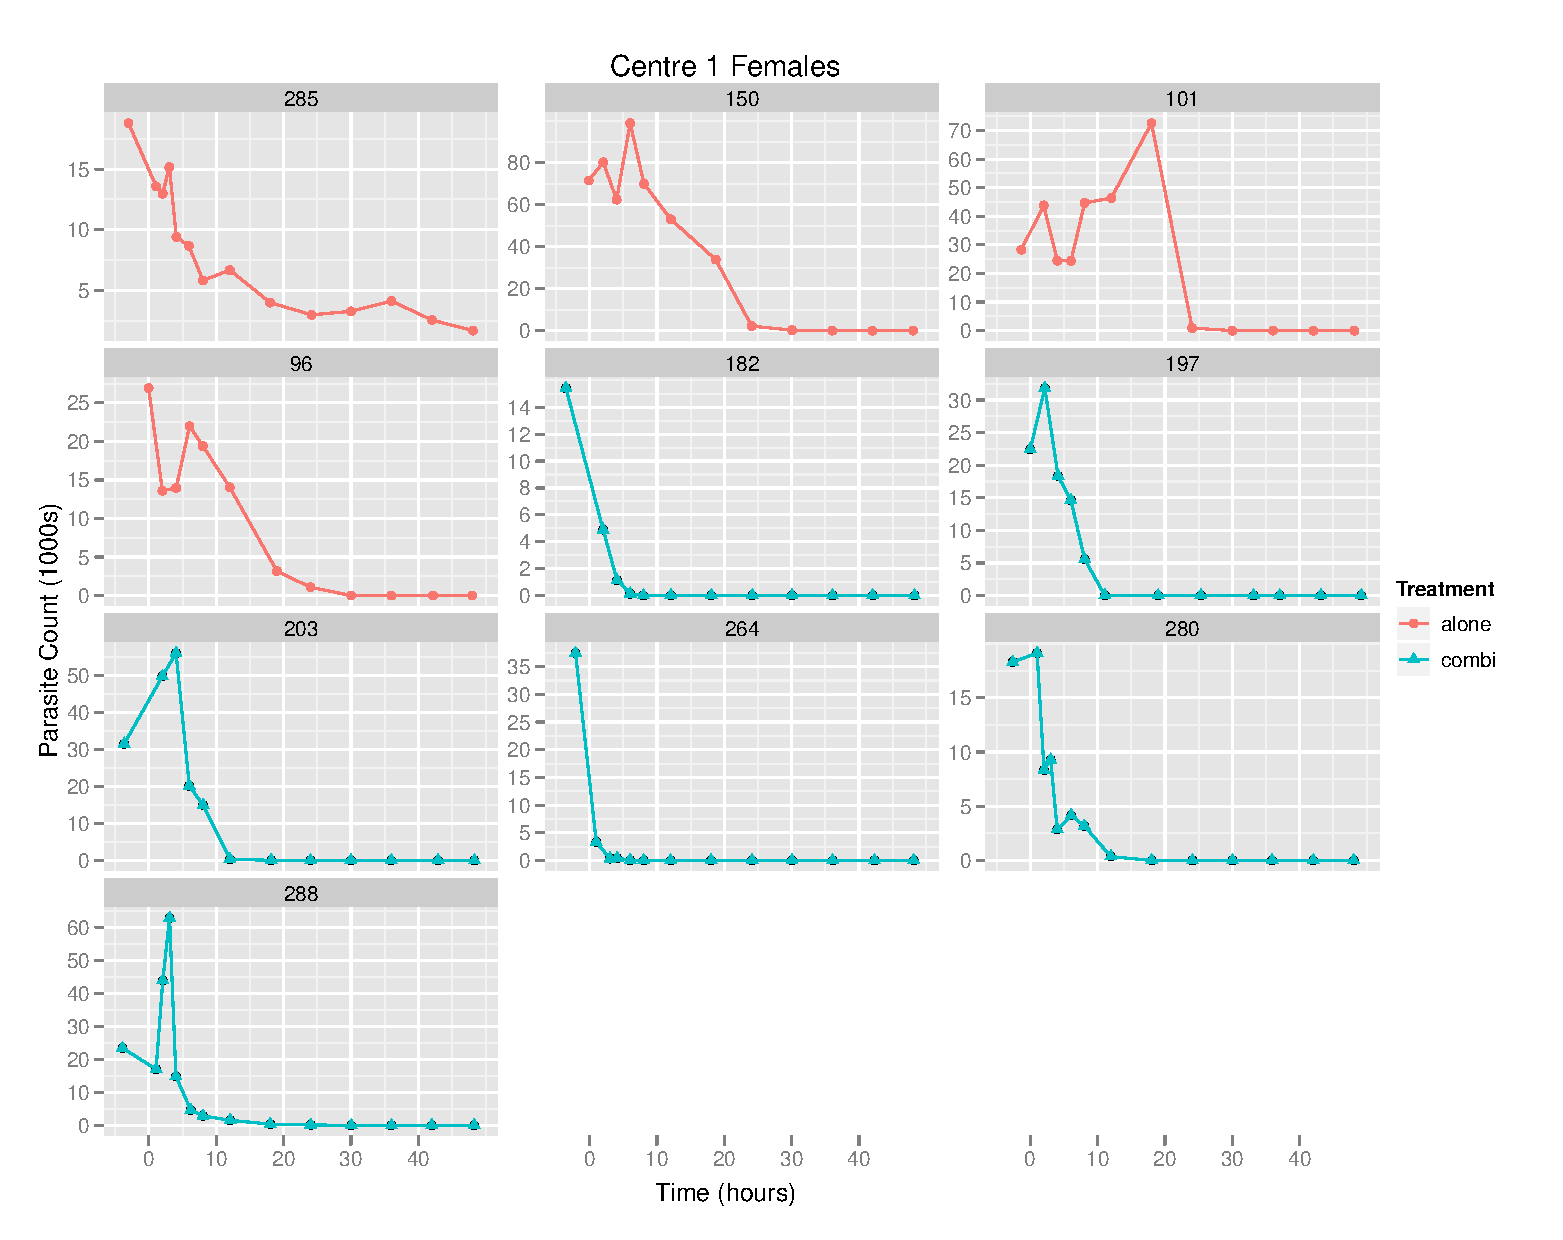
\includegraphics[width=6.1in]{raw1F.eps}
\caption{Parasite count for centre 1 females}\label{raw1F}
\end{figure} 
\begin{figure}[h]
\centering
\includegraphics[width=6.1in]{raw1M.eps}
\caption{Parasite count for centre 1 males}\label{raw1M}
\end{figure} 
\begin{figure}[h]
\centering
\includegraphics[width=6.1in]{raw2F.eps}
\caption{Parasite count for centre 2 females}\label{raw2F}
\end{figure} 
\begin{figure}[h]
\centering
\includegraphics[width=6.1in]{raw2M.eps}
\caption{Parasite count for centre 2 males}\label{raw2M}
\end{figure} 
\subsection{Main features of the data}
Generally, there appears to be a drop in the parasite count from an initial high level to zero or near zero within about 20 to 30 hours from first treatment. In some cases there is a rapid monotonic drop off within 10 hours. In other cases the \textit{recorded} parasite count fluctuates up and down before dropping to zero over a longer period.

To briefly summarise, the main behaviours observed are:
\begin{itemize}
\item A relatively steep monotonic drop in the count e.g. centre 1 female subjects 182 and 264 (Figure \ref{raw1F}), centre 1 male subjects 187, 162, 54, 176 and 185 (Figure \ref{raw1M}), centre 2 female subjects 462, 523 and 525 (Figure \ref{raw2F}) and centre 2 male subjects 509, 469 and 511 (Figure \ref{raw2M}).

A variation of this type comprises has the parasite count increasing after the first dose before falling e.g. subjects 197 and 203 (Figure \ref{raw1F}) and subjects 262 and 294 (Figure \ref{raw1M}). 
\item A more erratic and slower drop in the parasite count e.g. centre 1 female subjects 285 and 96 (Figure \ref{raw1F}), centre 1 male subjects 295 and 140 (Figure \ref{raw1M}) and centre 2 female subjects 521, 502 and 505 (Figure \ref{raw2F}). 
\item The parasite count seems to fluctuate about a constant level before falling e.g. centre 1 female subjects 150 and 101 (Figure \ref{raw1F}) and centre 1 male subjects 224, 98, 80 and 218 (Figure \ref{raw1M}). 
\end{itemize}
There are some profiles that we might suspect contain anomalous data such as subject 500 in Figure \ref{raw2M} where there are two unusually high values compared to the main trend. We might suspect that some inconsistency in the counting procedure explains these values rather than the patient's parasite count jumping by a large amount on these occasions. Therefore, we should start by looking at how the parasite count was obtained to give an insight into any potential sources of inconsistency.
\subsection{The Parasite Count}
One of the first questions addressed was whether the parasite count is a true count, and thus Poission statistics would be applicable, or whether it is a derived measurement. Our contact informed us that the method used to arrive at the \texttt{parct} values was that a microscopist would count a chosen area of a slide of blood, counting parasites ($N_p$) and white blood cells ($N_w$). The number of white blood cells in a $\mu L$ of blood ($\rho_w$) is automatically counted by a machine. Accordingly the number of parasites in a $\mu L$ of blood (\texttt{parct}) is given by:
$$\mathtt{parct}=\frac{N_p}{N_w}\rho_w$$
and thus we cannot treat this derived measurement as a count for modeling purposes.

We were also informed that the white blood cell count is right skewed and so we might expect that the parasite count per $\mu L$ will be also. Table \ref{predose} shows the pre-treatment parasite counts in the subjects from each test centre and of each sex. The $M^*$ row for centre 002 is where one large outlying value of 196029 has been removed. It can be seen that for 3 cases the mean is larger than the median meaning that the distributions are right skewed. This is to be expected for non-negative data such as this. When model fitting to this data we may have to choose some transformation of the parasite count such as taking logarithms.
\begin{table}[h]
\centering
\caption{Pre-dose parasite counts}\label{predose}
\begin{tabular}{|cc|cccccc|}
\hline
Centre&Sex&N&Mean&Median&SD&1st Qu.&3rd Qu.\\\hline
\multirow{2}{*}{001}&M&14&27060&20960&17820.9&16750&24830\\
&F&10&29410&25170&16221.2&19700&30700\\\hline
\multirow{3}{*}{002}&M&8&50540&23290&63679.9&12240&58290\\
&$M^*$&\textit{7}&\textit{29750}&\textit{20610}&\textit{26436.6}&\textit{11180}&\textit{38580}\\
&F&11&26110&27360&17262.4&11860&30400\\\hline
\end{tabular}
\end{table}
\pagebreak
\section{Preliminary Analysis}
\subsection{Deriving PC90}
The project specification says that the endpoint of primary importance is PC90, the time to achieve a reduction of the parasitaemia by 90\% of baseline level. As a first attempt at deriving estimates of PC90 from the data, simple linear polynomial fits to the logarithm of the parasite count with time from first dose were investigated (actually log(1+parct)).

It was found that a cubic was the most suitable model if we include the data only up to the first 0 parasite count. For some patients where the parasite count drops quickly to 0. A fit that includes the subsequent run of 0s would pull the cubic fit away from the most sensible estimate of PC90. It is more suitable for the purpose of estimating PC90 to only model the drop in the count to 0 using a simple cubic model. 

Figure \ref{cubics} shows the cubic fits to the log parasite count for the 43 subjects treated. The horizontal dotted line on the plots shows the PC90 level i.e. where the parasite count has fallen to 10\% of its initial value. The value of PC90 i.e. the time t at which the parasite count has fallen to 10\% was found by least-squares i.e. using the \texttt{optimize} function in R to minimise:
$$[log(1+0.1P_0)-\beta_0-\beta_1t-\beta_2t^2-\beta_3t^3]^2$$
where $P_0$ is the pre-treatment parasite count, $t$ is the time from first dose and $\beta_i$ are the fitted coefficients for the models for each of the 43 patients. Table \ref{pc90} shows the values of PC90 derived from the cubic fit to the parasite count by centre, sex and treatment.
\begin{sidewaysfigure}[p]
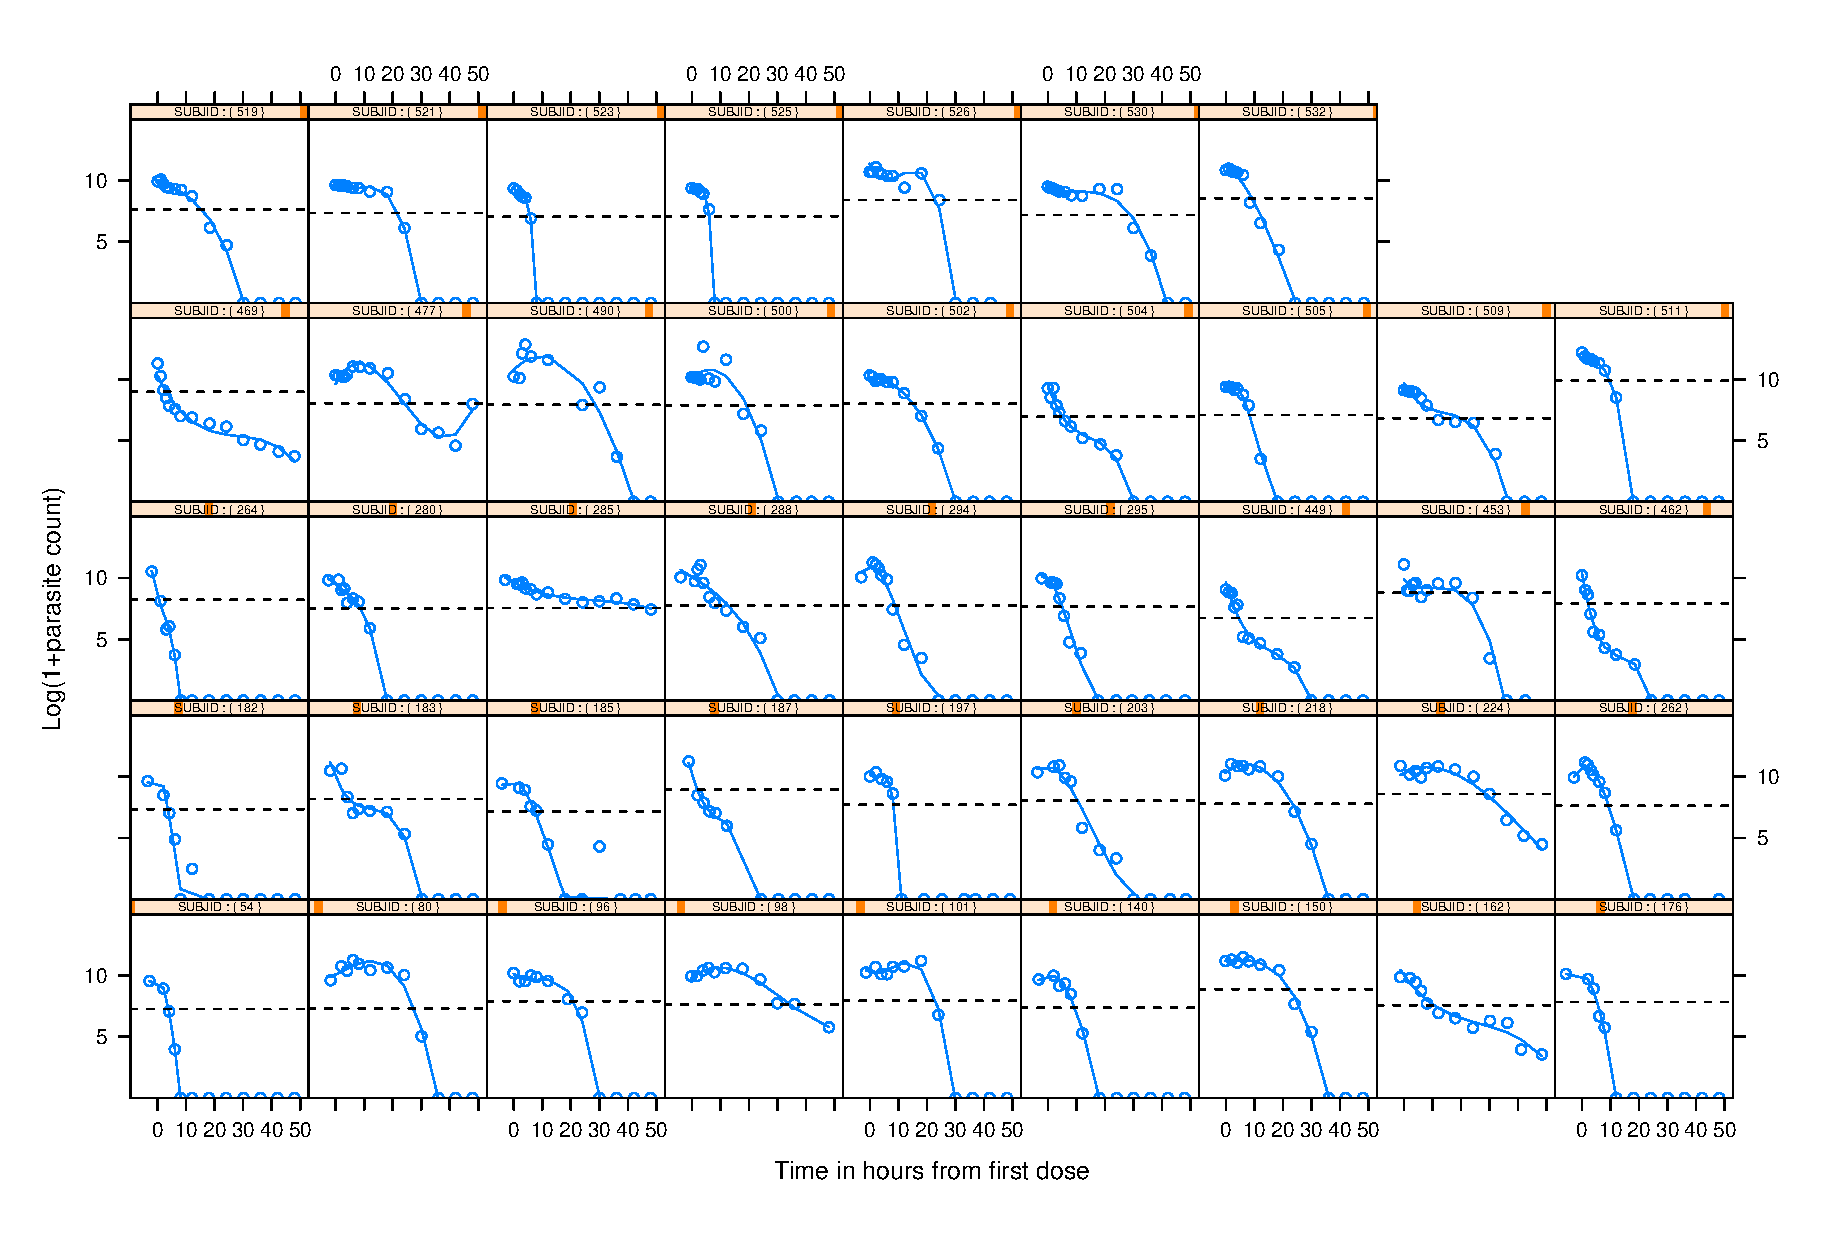
\includegraphics[scale=0.8]{cubics.eps} 
\caption{Cubic fits to log parasite count vs. time from first dose for 43 subjects treated}\label{cubics}
\end{sidewaysfigure}
\begin{table}[h]
\centering
\caption{Derived PC90 values}\label{pc90}
\begin{tabular}{|cc|c|c|}
\hline
&&\multicolumn{2}{c|}{Treatment}\\
Centre&Sex&A&B\\\hline
\multirow{2}{*}{001}&M&$\begin{array}{c}3.8,\ 27.9,\ 34.3,\  9.8,\\5.0,\  0.8,\ 28.9,\  4.7\end{array}$&$\begin{array}{c}9.5,\  5.3,\  7.7,\\23.5,\  9.4,\  8.1\end{array}$\\\cline{2-4}
&F&$\begin{array}{c}21.1,\ 23.2,\\22.5,\ 47.2\end{array}$&$\begin{array}{c}4.2,\ 8.6 ,\ 9.4,\\0.9,\ 8.6,\ 12.9\end{array}$\\\hline
\multirow{2}{*}{002}&M&$\begin{array}{c}4.5,\ 2.1,\\20.6,\ 29.1\end{array}$&$\begin{array}{c}19.3,\ 10.0,\\15.6,\ 8.9\end{array}$\\\cline{2-4}
&F&$\begin{array}{c}20.1,\ 2.2,\ 24.0,\ 28.7,\\5.0,\ 22.2,\ 23.7\end{array}$&$\begin{array}{c}15.4,\  8.4,\\5.9,\ 6.3\end{array}$\\\hline
\end{tabular}
\end{table}
\subsection{PC90 ANOVA} 
3-way ANOVA with interactions was performed on the PC90 data over centre, sex and treatment. The results are shown in Table \ref{anova}. It can be seen that the only significant effect on PC90 is the treatment used (\texttt{trt}), with perhaps some effect of the interaction between sex and treatment. This is a result we might expect. If we fit a model with treatment as the only factor we find that treatment B reduces the PC90 time compared to treatment A by 8.0 hours with a 95\% confidence interval of (1.9, 14.1) hours.
\begin{table}[h]
\centering
\caption{3-way ANOVA with interactions for PC90}\label{anova}
\begin{boxedverbatim}
Response: PC90
                                         Df Sum Sq Mean Sq F value  Pr(>F)  
factor(SEX)                               1   49.4    49.4  0.5218 0.47488  
factor(CENTREID)                          1    0.1     0.1  0.0008 0.97816  
factor(trt)                               1  697.5   697.5  7.3708 0.01022 *
factor(SEX):factor(CENTREID)              1   57.4    57.4  0.6062 0.44146  
factor(SEX):factor(trt)                   1  389.4   389.4  4.1151 0.05016 .
factor(CENTREID):factor(trt)              1  143.4   143.4  1.5150 0.22658  
factor(SEX):factor(CENTREID):factor(trt)  1   49.3    49.3  0.5214 0.47505  
Residuals                                35 3312.0    94.6
\end{boxedverbatim}
\end{table}

Diagnostic plots of the residuals of the ANOVA model are shown in Figure \ref{resid}. There does not seem to be any significant departure from normality in the distribution of residuals which suggests that we may not need a transformation for modelling the PC90 data. However, there is perhaps some evidence of heteroskedasticity in that the variance of the residuals appears to increase with increasing fitted PC90 value, hence we may need a variance-stabalising transformation.
\begin{sidewaysfigure}[p]
\centering
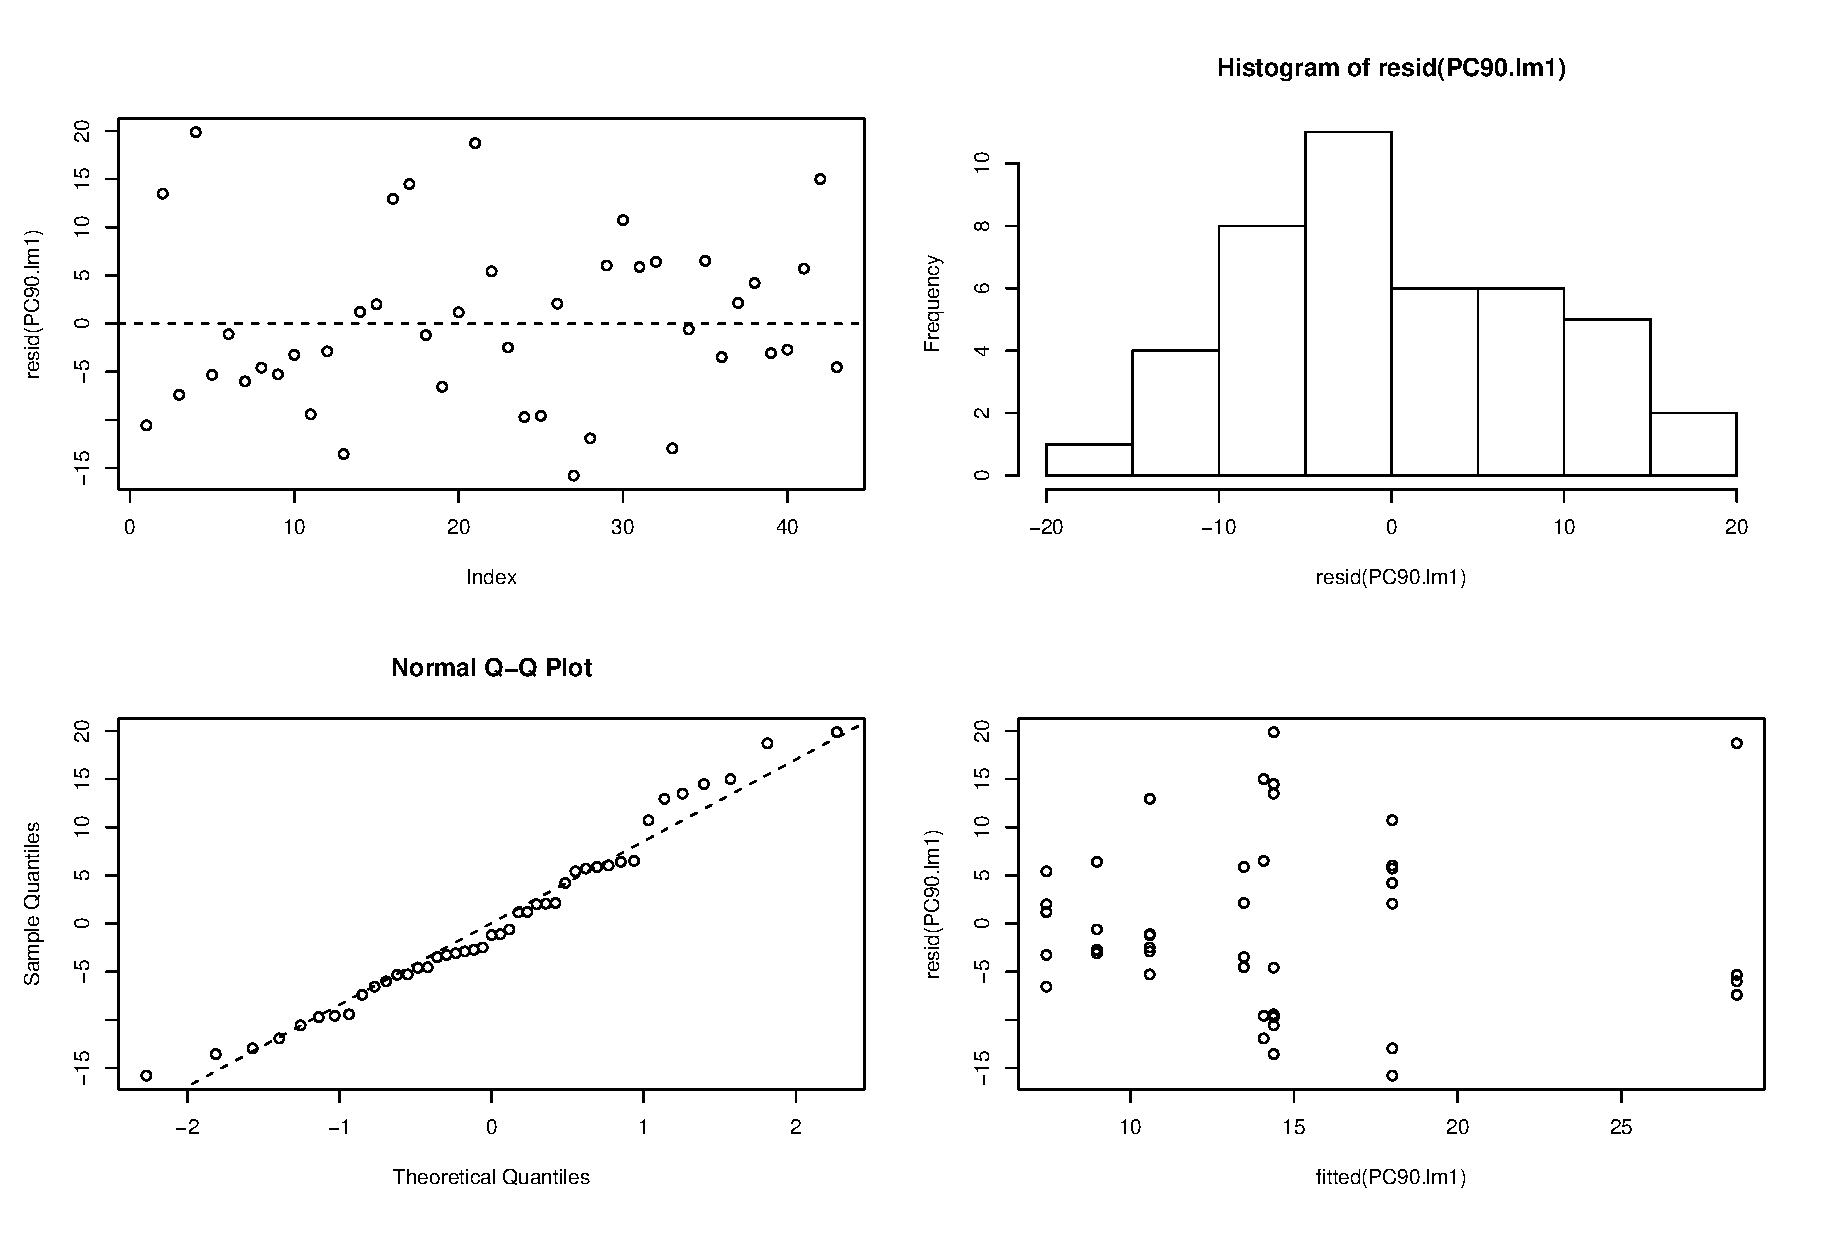
\includegraphics[scale=0.8]{PC90diag.eps}
\caption{Residuals for ANOVA on PC90}\label{resid}
\end{sidewaysfigure}
\section{Work Plan}
The next stages of the analysis are:
\begin{itemize}
\item Look in more detail at deriving the PC90 estimates. Logistic regression has been suggested in the project outline which would require non-linear regression techniques.
\item Look at how to identify and deal with suspicious outliers in the parasite count data and how they influence our estimates of PC90.
\item Incorporate the error in PC90 estimates into the modelling of treatment effect.
\end{itemize}